\subsection*{Daglig helbredstilstand}
Førend en træning påbegyndes skal brugerens daglige helbredstilstand angives. Dette er for at sikre, at træningen tilpasses den individuelle bruger samt imødekomme dag til dag variationer. Af \autoref{fig:helbredstilstand} fremgår aktivitetsdiagrammet for angivelse af den daglige helbredstilstand. 

\begin{figure} [H]
\centering
\textbf{Aktivitetsdiagram: Daglig helbredstilstand}\par\medskip
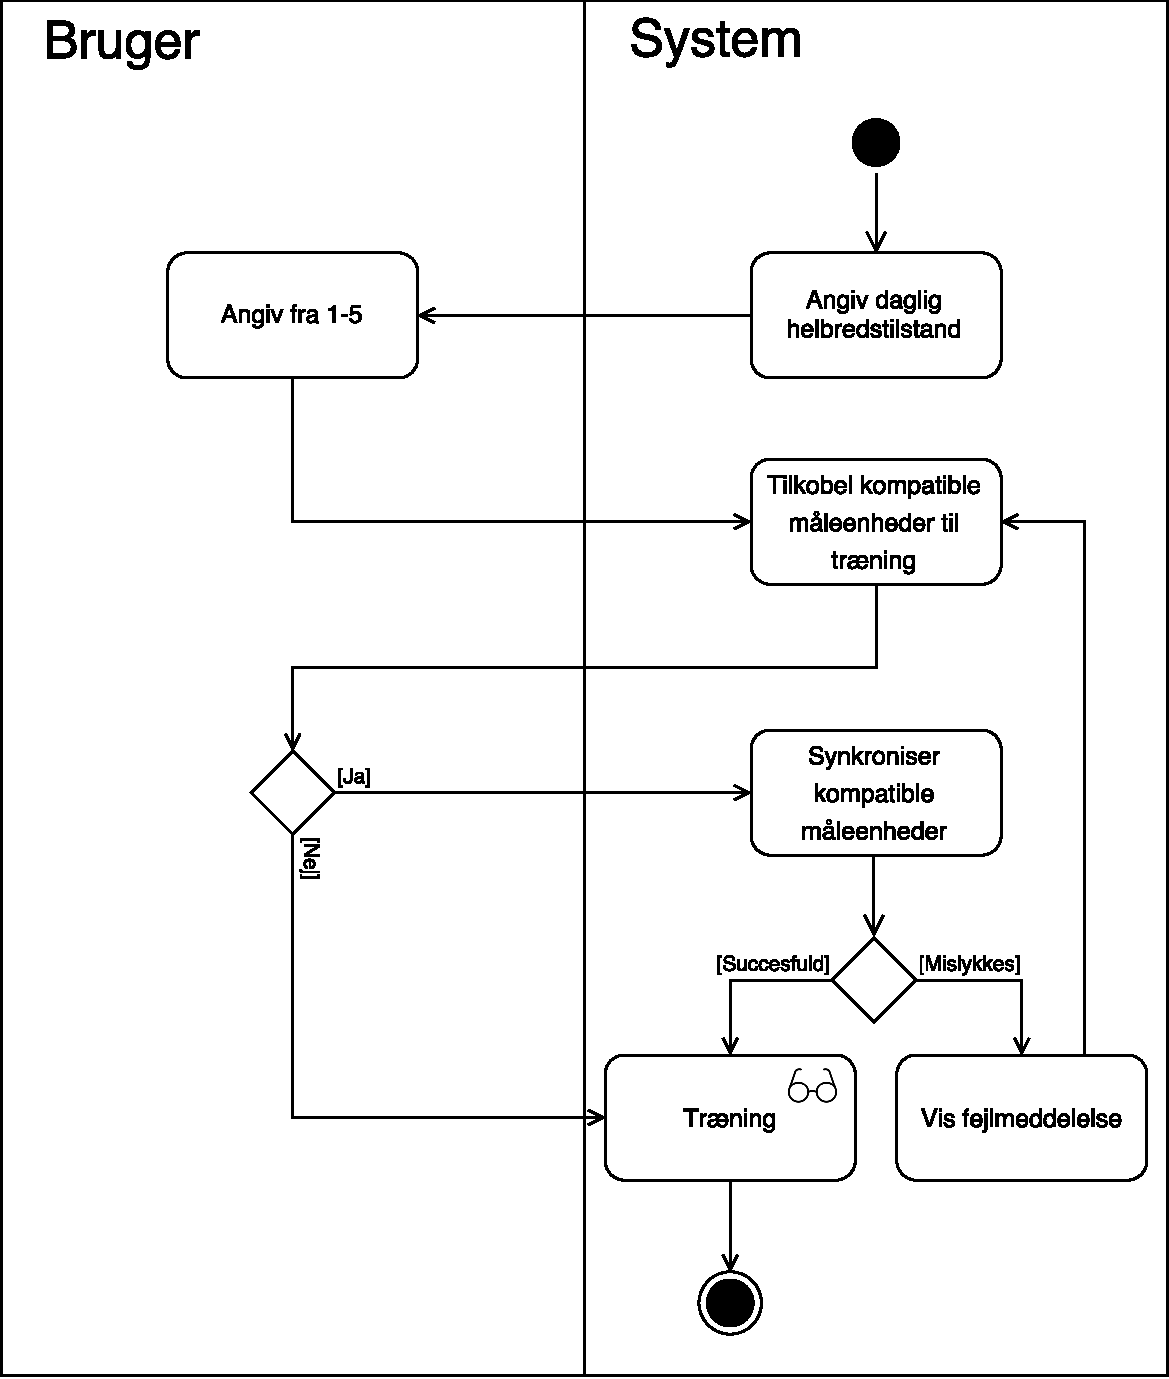
\includegraphics[width=0.9\textwidth]{figures/aktivitetsdiagram/NYHelbredstilstand}
\caption{Aktivitetsdiagram for daglig helbredstilstand. Træning er yderligere beskrevet af \autoref{fig:traening}.}
\label{fig:helbredstilstand}
\end{figure}

\noindent
Den daglige helbredtilstand angives ved hjælp af en skala fra 1, svarende til en dårlig helbredstilstand, til 5, svarende til en god helbredstilstand. Herefter skal brugeren angive om der ønskes at tilkobles kompatible enheder til systemt, eksempelvis pulsmåler. Vælger brugeren ikke at tilkoble eksterne enheder, startes timer og GPS, hvorefter selve træningen påbegyndes. Vælger brugeren at tilkoble enheder, prøver systemet at synkronisere med enhederne. Lykkes dette ikke, sender systemet en fejlmeddelelse, og brugeren skal igen angive om der ønskes at tilkoble kompatible enheder til systemet. 
Hvis det lykkes kan brugeren fortsætte træningen, som yderligere er beskrevet i \autoref{fig:traening}. 


%Ud fra den daglige helbredstilstand, kategoriseringen af KOL samt evaluering fra førhenværende træning, passende til den angivede helbredstilstand, vælges et træningsniveau passende til brugerens nuværende helbred. Dertil foreslås brugeren forskellige træningsformer, herunder konditions-, styrketræning samt vejrtrækningsøvelser. Den ønskede træningsform vælges, hvortil træningen kan udføres. Træningen er yderligere beskrevet af \autoref{fig:traening}. 